
\documentclass[12pt]{article}

\usepackage[a4paper,margin=1in]{geometry}
\usepackage{tikz}
\usetikzlibrary{arrows.meta, positioning}
\usepackage{longtable}
\usepackage{booktabs}
\usepackage{enumitem}
\usepackage[hidelinks]{hyperref}

\title{\textbf{Structured Analysis and Structured Design (SA/SD)}\\
Software Component Cataloguing System}
\author{Prepared by: Priyank Bansal}
\date{\today}

\setlength{\parindent}{0pt}
\setlength{\parskip}{0.6em}

\begin{document}
\maketitle
\tableofcontents
\newpage

\section{Description}
This document presents the Structured Analysis and Structured Design (SA/SD) of the Software Component Cataloguing System. It focuses on the system structure, flow of information, module boundaries, and maintainable design.

\subsection{Purpose}
The purpose of this document is to describe the software in a structured form so that the relationship between functions, processes, data, and modules can be clearly understood.

\subsection{Scope}
The system is a web-based catalogue for reusable software components. It supports registration, login, component storage, catalogue organization, searching, and usage tracking.

\subsection{Maintenance and Context}
The design must remain easy to update when new component fields, search filters, catalogue categories, or reporting features are added. The application should therefore be divided into clear modules with minimal dependency between them.

\section{Development Plan}

\subsection{Analysis Phase}
The system is first analyzed by identifying the external user, the major functions, and the data exchanged between the user and the system. The main outcome of this phase is the functional breakdown and the context-level view.

\subsection{Design Phase}
The analyzed functions are then converted into modules, data structures, and deployment layers. The main goal is to keep the design simple, modular, and easy to maintain.

\subsection{Maintenance Plan}
The design should support future enhancement without major restructuring. For example, additional metadata fields or improved search logic should be added with small changes only.

\section{Target Users}
\begin{itemize}[leftmargin=1.2cm]
    \item \textbf{User / Developer}: registers, logs in, searches components, and manages catalogue entries.
    \item \textbf{Admin}: oversees stored records and monitors catalogue-related information.
\end{itemize}

\section{Features}

\subsection{Functional Decomposition}
The system can be divided into the following major functions:

\begin{center}
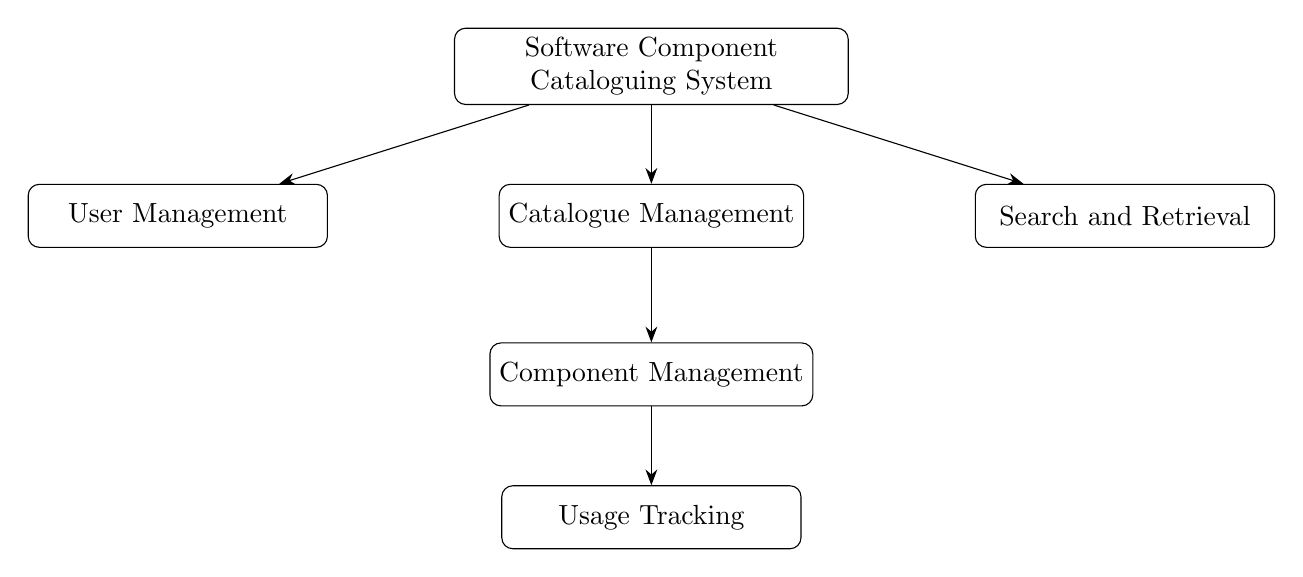
\begin{tikzpicture}[
    node distance=10mm and 16mm,
    box/.style={draw, rounded corners, align=center, minimum width=5.0cm, minimum height=0.95cm},
    sub/.style={draw, rounded corners, align=center, minimum width=3.8cm, minimum height=0.8cm}
]
\node[box] (root) {Software Component\\Cataloguing System};

\node[sub, below left=of root] (u) {User Management};
\node[sub, below=of root] (c) {Catalogue Management};
\node[sub, below right=of root] (s) {Search and Retrieval};

\node[sub, below=of c, yshift=-2mm] (m) {Component Management};
\node[sub, below=of m] (t) {Usage Tracking};

\draw[-{Stealth[length=2mm]}] (root) -- (u);
\draw[-{Stealth[length=2mm]}] (root) -- (c);
\draw[-{Stealth[length=2mm]}] (root) -- (s);
\draw[-{Stealth[length=2mm]}] (c) -- (m);
\draw[-{Stealth[length=2mm]}] (m) -- (t);
\end{tikzpicture}
\end{center}

\subsection{Context Diagram}
The context diagram shows the system as a single process interacting with the external user.

\begin{center}
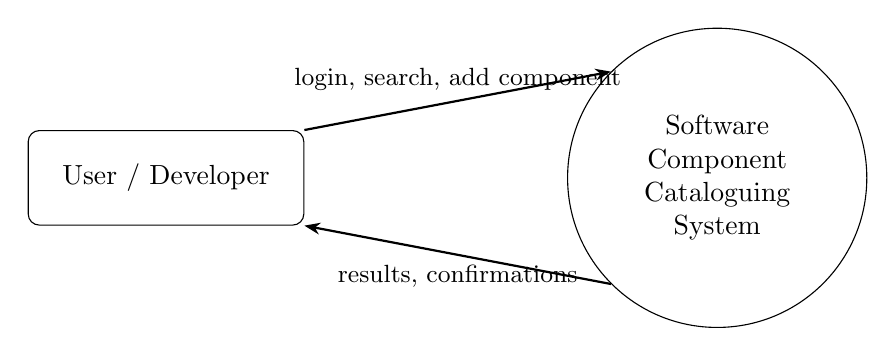
\begin{tikzpicture}[
    entity/.style={draw, rounded corners, align=center, minimum width=3.5cm, minimum height=1.2cm},
    process/.style={draw, circle, align=center, minimum size=3.8cm},
    flow/.style={-{Stealth[length=2mm]}, thick}
]

\node[entity] (user) at (-5,0) {User / Developer};
\node[process] (sys) at (2,0) {Software\\Component\\Cataloguing\\System};

\draw[flow] (user.north east) -- node[above, font=\small] {login, search, add component} (sys.north west);
\draw[flow] (sys.south west) -- node[below, font=\small] {results, confirmations} (user.south east);

\end{tikzpicture}
\end{center}

\subsection{DFD Level 1}
The system is divided into the following high-level processes:
\begin{enumerate}[leftmargin=1.2cm]
    \item Authenticate User
    \item Manage Catalogue
    \item Manage Component Records
    \item Search Components
    \item Track Usage
\end{enumerate}

\begin{center}
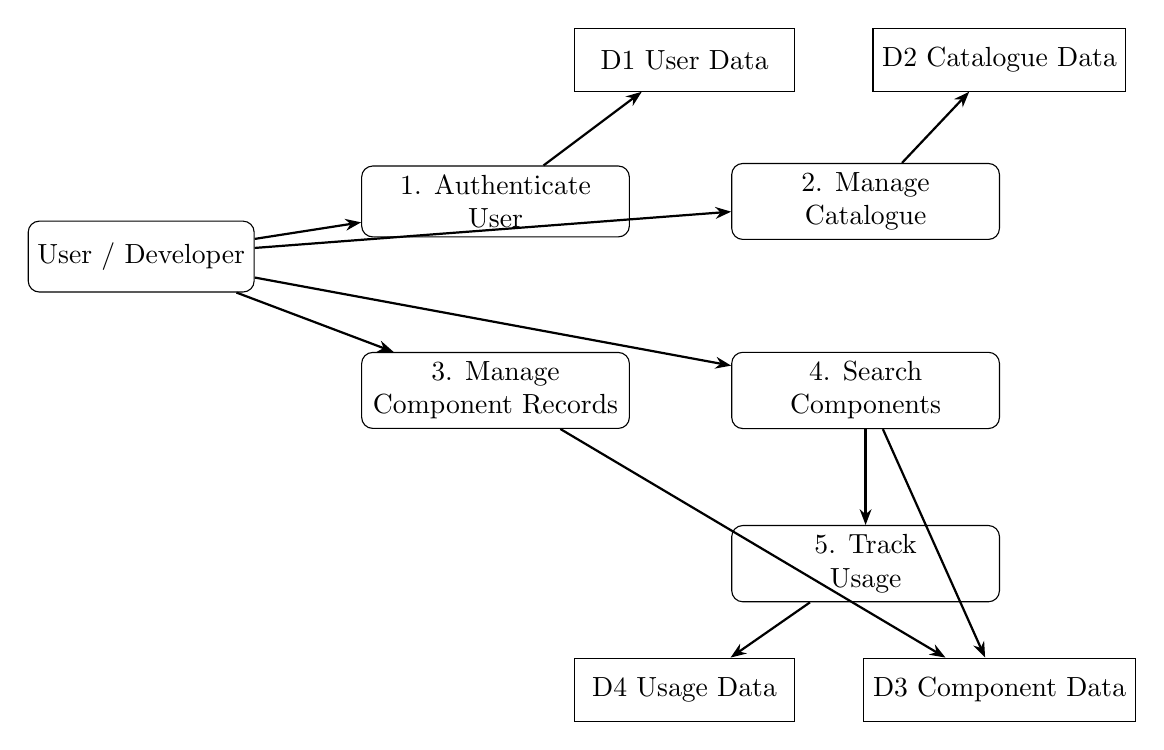
\begin{tikzpicture}[
    entity/.style={draw, rounded corners, align=center, minimum width=2.8cm, minimum height=0.9cm},
    process/.style={draw, rounded corners, align=center, minimum width=3.4cm, minimum height=0.9cm},
    store/.style={draw, minimum width=2.8cm, minimum height=0.8cm, align=center},
    flow/.style={-{Stealth[length=2mm]}, thick}
]
\node[entity] (user) at (-6,1.5) {User / Developer};

\node[process] (p1) at (-1.5,2.2) {1. Authenticate\\User};
\node[process] (p2) at (3.2,2.2) {2. Manage\\Catalogue};
\node[process] (p3) at (-1.5,-0.2) {3. Manage\\Component Records};
\node[process] (p4) at (3.2,-0.2) {4. Search\\Components};
\node[process] (p5) at (3.2,-2.4) {5. Track\\Usage};

\node[store] (d1) at (0.9,4.0) {D1 User Data};
\node[store] (d2) at (4.9,4.0) {D2 Catalogue Data};
\node[store] (d3) at (4.9,-4.0) {D3 Component Data};
\node[store] (d4) at (0.9,-4.0) {D4 Usage Data};

\draw[flow] (user) -- (p1);
\draw[flow] (p1) -- (d1);

\draw[flow] (user) -- (p2);
\draw[flow] (p2) -- (d2);

\draw[flow] (user) -- (p3);
\draw[flow] (p3) -- (d3);

\draw[flow] (user) -- (p4);
\draw[flow] (p4) -- (d3);

\draw[flow] (p4) -- (p5);
\draw[flow] (p5) -- (d4);
\end{tikzpicture}
\end{center}

\subsection{Process Flow Descriptions}

\textbf{Authentication Flow}
\begin{enumerate}[leftmargin=1.2cm]
    \item The user enters login or registration information.
    \item The system validates the input.
    \item If valid, the user is authenticated.
    \item If invalid, an error message is displayed.
\end{enumerate}

\textbf{Add Component Flow}
\begin{enumerate}[leftmargin=1.2cm]
    \item The user opens the component entry page.
    \item The user enters component details.
    \item The system validates the data.
    \item Valid data is stored in the database.
    \item A confirmation message is displayed.
\end{enumerate}

\textbf{Search Component Flow}
\begin{enumerate}[leftmargin=1.2cm]
    \item The user enters a search query.
    \item The system searches the stored records.
    \item Matching records are retrieved.
    \item The results are displayed to the user.
\end{enumerate}

\subsection{Data Dictionary}
\begin{longtable}{p{3.4cm}p{3cm}p{7cm}}
\toprule
\textbf{Data Item} & \textbf{Type} & \textbf{Description} \\
\midrule
UserID & Integer & Unique identifier for each user \\
Username & String & Login and display name \\
Email & String & User email address \\
Password & String & Authentication credential \\
CatalogueID & Integer & Unique identifier for a catalogue \\
CatalogueName & String & Name of the catalogue \\
ComponentID & Integer & Unique identifier for a component \\
ComponentName & String & Name of the software component \\
Description & Text & Component details and notes \\
Keywords & String & Search terms for retrieval \\
UsageCount & Integer & Number of times a component is used \\
\bottomrule
\end{longtable}

\section{Technologies}

\subsection{System Architecture}
The system follows a three-tier architecture.

\begin{center}
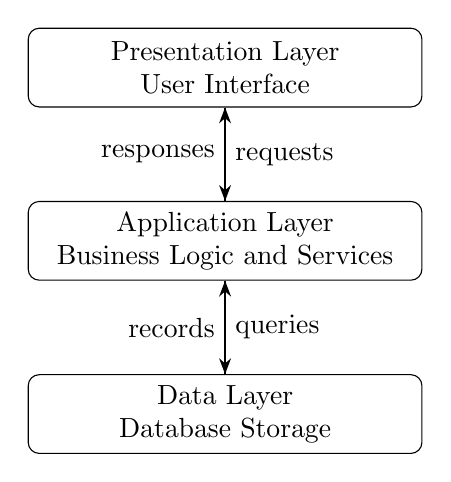
\begin{tikzpicture}[
    box/.style={draw, rounded corners, align=center, minimum width=5cm, minimum height=1cm},
    flow/.style={-{Stealth[length=2mm]}, thick}
]
\node[box] (front) at (0,2.2) {Presentation Layer\\User Interface};
\node[box] (mid) at (0,0) {Application Layer\\Business Logic and Services};
\node[box] (data) at (0,-2.2) {Data Layer\\Database Storage};

\draw[flow] (front) -- node[right]{requests} (mid);
\draw[flow] (mid) -- node[right]{queries} (data);
\draw[flow] (data) -- node[left]{records} (mid);
\draw[flow] (mid) -- node[left]{responses} (front);
\end{tikzpicture}
\end{center}

\subsection{Module Design}
The system is organized into the following modules:
\begin{itemize}[leftmargin=1.2cm]
    \item \textbf{Authentication Module}: handles registration and login.
    \item \textbf{Catalogue Module}: manages catalogue creation and organization.
    \item \textbf{Component Module}: stores and updates component records.
    \item \textbf{Search Module}: handles keyword search and result retrieval.
    \item \textbf{Usage Module}: tracks component access and reuse.
\end{itemize}

\subsection{Control Flow}
\textbf{Login Control Flow}
\begin{enumerate}[leftmargin=1.2cm]
    \item Enter credentials.
    \item Validate credentials.
    \item Grant or deny access.
\end{enumerate}

\textbf{Component Control Flow}
\begin{enumerate}[leftmargin=1.2cm]
    \item Enter component details.
    \item Validate details.
    \item Save or reject the record.
\end{enumerate}

\textbf{Search Control Flow}
\begin{enumerate}[leftmargin=1.2cm]
    \item Accept search query.
    \item Match query against stored data.
    \item Return matching results.
\end{enumerate}

\section{Distribution Plan}
\subsection{Deployment View}
The system is deployed as a web application.
\begin{itemize}[leftmargin=1.2cm]
    \item Users access the system through a browser.
    \item The frontend communicates with backend services.
    \item The backend stores data in the database.
\end{itemize}

\subsection{Maintenance Plan}
\begin{itemize}[leftmargin=1.2cm]
    \item The modular structure supports future extension.
    \item New component attributes can be added with minimal changes.
    \item Search and reporting logic can be improved independently.
\end{itemize}

\section{Conclusion}
This SA/SD document provides the structural view of the Software Component Cataloguing System. It includes the functional decomposition, context diagram, DFD Level 1, process flows, data dictionary, architecture, module design, and maintenance planning needed for submission.

\end{document}
